
%% bare_conf.tex
%% V1.4b
%% 2015/08/26
%% by Michael Shell
%% See:
%% http://www.michaelshell.org/
%% for current contact information.
%%
%% This is a skeleton file demonstrating the use of IEEEtran.cls
%% (requires IEEEtran.cls version 1.8b or later) with an IEEE
%% conference paper.
%%
%% Support sites:
%% http://www.michaelshell.org/tex/ieeetran/
%% http://www.ctan.org/pkg/ieeetran
%% and
%% http://www.ieee.org/

%%*************************************************************************
%% Legal Notice:
%% This code is offered as-is without any warranty either expressed or
%% implied; without even the implied warranty of MERCHANTABILITY or
%% FITNESS FOR A PARTICULAR PURPOSE!
%% User assumes all risk.
%% In no event shall the IEEE or any contributor to this code be liable for
%% any damages or losses, including, but not limited to, incidental,
%% consequential, or any other damages, resulting from the use or misuse
%% of any information contained here.
%%
%% All comments are the opinions of their respective authors and are not
%% necessarily endorsed by the IEEE.
%%
%% This work is distributed under the LaTeX Project Public License (LPPL)
%% ( http://www.latex-project.org/ ) version 1.3, and may be freely used,
%% distributed and modified. A copy of the LPPL, version 1.3, is included
%% in the base LaTeX documentation of all distributions of LaTeX released
%% 2003/12/01 or later.
%% Retain all contribution notices and credits.
%% ** Modified files should be clearly indicated as such, including  **
%% ** renaming them and changing author support contact information. **
%%*************************************************************************


% *** Authors should verify (and, if needed, correct) their LaTeX system  ***
% *** with the testflow diagnostic prior to trusting their LaTeX platform ***
% *** with production work. The IEEE's font choices and paper sizes can   ***
% *** trigger bugs that do not appear when using other class files.       ***
%                       ***
% The testflow support page is at:
% http://www.michaelshell.org/tex/testflow/



\documentclass[conference]{IEEEtran}


% *** CITATION PACKAGES ***
%
%\usepackage{cite}
% cite.sty was written by Donald Arseneau
% V1.6 and later of IEEEtran pre-defines the format of the cite.sty package
% \cite{} output to follow that of the IEEE. Loading the cite package will
% result in citation numbers being automatically sorted and properly
% "compressed/ranged". e.g., [1], [9], [2], [7], [5], [6] without using
% cite.sty will become [1], [2], [5]--[7], [9] using cite.sty. cite.sty's
% \cite will automatically add leading space, if needed. Use cite.sty's
% noadjust option (cite.sty V3.8 and later) if you want to turn this off
% such as if a citation ever needs to be enclosed in parenthesis.
% cite.sty is already installed on most LaTeX systems. Be sure and use
% version 5.0 (2009-03-20) and later if using hyperref.sty.
% The latest version can be obtained at:
% http://www.ctan.org/pkg/cite
% The documentation is contained in the cite.sty file itself.


% *** GRAPHICS RELATED PACKAGES ***
%
\ifCLASSINFOpdf \usepackage[pdftex]{graphicx} \usepackage{wrapfig} % declare the
% path(s) where your graphic files are
\graphicspath{{pic/}} % and their extensions so you won't have to specify these
% with
% every instance of \includegraphics
\DeclareGraphicsExtensions{.png} \else % or other class option (dvipsone,
% dvipdf, if not using dvips). graphicx
% will default to the driver specified in the system graphics.cfg if no
% driver is specified.
% \usepackage[dvips]{graphicx}
% declare the path(s) where your graphic files are
% \graphicspath{{../eps/}}
% and their extensions so you won't have to specify these with
% every instance of \includegraphics
% \DeclareGraphicsExtensions{.eps}
\fi

% correct bad hyphenation here
\hyphenation{op-tical net-works semi-conduc-tor}

\usepackage{textcomp} \newcommand{\toolname}{Perquimans?!} \begin{document}
	\title{A Tool for Visualizing Patterns of Spreadsheet Function Combinations}
	
	
	% author names and affiliations
	% use a multiple column layout for up to three different
	% affiliations
	\author{ \IEEEauthorblockN{Justin A. Middleton, Emerson Murphy-Hill}
		\IEEEauthorblockA{North Carolina State University\\ Raleigh, North Carolina,
			USA} }
	
	% use for special paper notices
	%\IEEEspecialpapernotice{(Invited Paper)}
	
	% make the title area
	\maketitle
	
	\begin{figure*}[t] 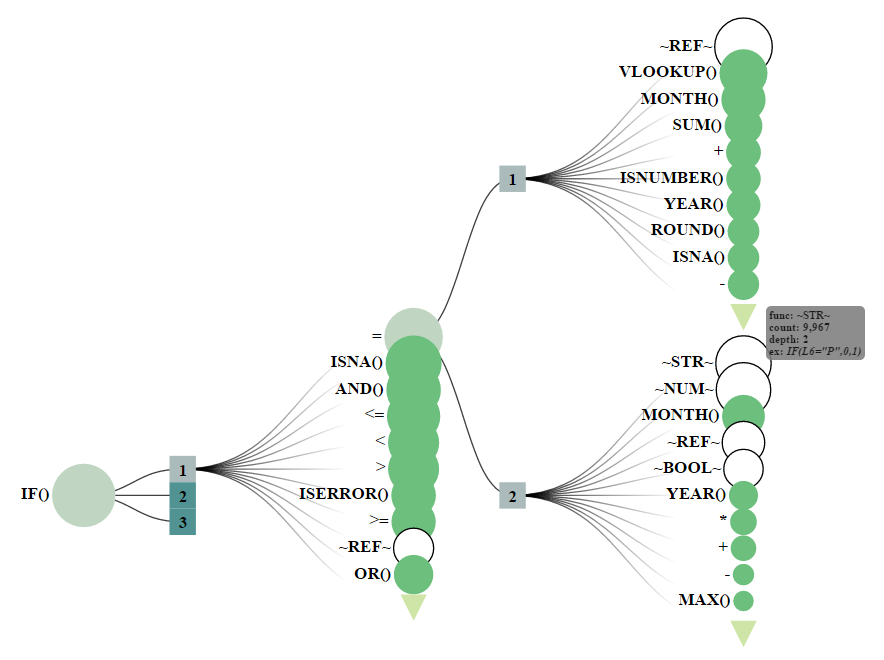
\includegraphics[width = \textwidth]{IFargslabel} \caption{A
			picture of \toolname} \centering \label{fig:fullpic} \end{figure*}
	
	% As a general rule, do not put math, special symbols or citations
	% in the abstract
	\begin{abstract} Spreadsheet environments often come equipped with an abundance
		of functions and operations to manipulate data, but it can be difficult to
		understand how programmers actually use these in practice. Furthermore, users
		can combine several functions into a complex formula, complicating matters for
		both researchers and practitioners who want to study formulae to improve
		spreadsheet practices. Therefore, we developed a tool that visualizes patterns
		of function combination in spreadsheets as an interactive tree of
		possibilities. Using spreadsheets from the public spreadsheet corpora, we then
		apply to the tool to real datasets and demonstrate its ability to capture the
		most common and most anomalous patterns of function combination and their
		contexts in actual workbooks. \end{abstract}
	
	\section{Introduction} Spreadsheets surround us, ordering the ever-growing
	flood of data that we produce. They serve key roles in industry, where as much
	as 95\% of U.S. financial firms use them daily \cite{panko2008sarbanes}, and
	academia, where teachers can use them to track research and students' grades,
	not to mention many other lines of work \cite{ko2011state}. It's this
	flexibility that grants them their allure: while a novice can still work
	without much experience, spreadsheets offer hundreds of specialized functions
	to fulfill a wide range of advanced needs, from complex statistics to text
	manipulation \cite{nardi1990spreadsheet}. As such, it should be no surprise
	that tens of millions of workers rely on these programs every day
	\cite{scaffidi2005estimating}.
	
	However, this ubiquity is not without danger: as more people adopt these tools
	and make larger and more complex sheets, the cost of failure grows too. To
	stress this, the European Spreadsheet Risks Interest Group (EuSpRIG) documents
	many horror stories of spreadsheets gone terribly
	wrong\footnote{http://www.eusprig.org/horror-stories.htm}. One such story tells
	of a 2013 economics paper which drew stark connections between debt and
	national growth. Its findings shaped many political initiatives throughout the
	United States and Europe. However, other researchers soon discovered that a
	critical coding error in the research spreadsheets hampered the results and
	that, by correcting this error, they completely reversed the findings! And this
	is only one of several accounts; even if most spreadsheet errors are relatively
	benign, poor spreadsheet practice can risk millions, if not billions, of
	dollars \cite{powell2009impact}.
	
	From these stories, we can see the dire importance of understanding how people
	actually use spreadsheets, if only to avoid disasters. Fortunately, spreadsheet
	researchers have supported this by amassing spreadsheet collections from
	diverse sources, industrial to academic. Collections like EUSES
	\cite{fisher2005euses}, Fuse \cite{barik2015fuse}, and the Enron corpus
	\cite{hermans2015enron} have already fueled productive research across the
	field, such as in Hermans' \cite{hermans2012detecting} or Jansen's
	\cite{jansen2015code} search for code smells\footnote{Or, instances of
		inelegant code that do not necessarily cause problems alone but nevertheless
		suggest a need for refactoring to prevent future problems. More on this in
		section IV.} in spreadsheet environments or Aivaloglou and colleague's work on
	making a grammar to capture every possible spreadsheet program in Excel
	\cite{aivaloglou2015grammar}. Additionally, some research has focused simply on
	comparing these collections, as Jansen did in 2015, to discover variation in
	spreadsheet techniques over time and location \cite{jansen2015enron}.
	
	Considering the sheer value of spreadsheets and all of these resources to
	describe their use, it becomes necessary that we design tools to make sense of
	it all. Tools, then, that empower people to explore datasets are rife with the
	potential to improve the current design of spreadsheets themselves and educate
	new generations of spreadsheets users on how to work best.
	
	This paper contributes such a tool, \toolname, that attempts to fulfill this by
	building on the aforementioned spreadsheet corpora. Working with spreadsheets
	in Excel, \toolname focuses primarily on the functions, like SUM and IF and
	hundreds more, which are the building blocks of formula and programs which
	determine values across a spreadsheet. The tool creates an interactive,
	exploratory visualization which captures how people combine these functions in
	a selected collection of spreadsheets, quantifying the broad patterns of
	function nesting while also being specific enough to find anomalous formulae
	and link them back to the specific cell in spreadsheets where they originate.
	\par
	
	Alongside the tool, we discuss several of the key decisions we faced during
	design, such as what to do with redundant formulae in a sheet or how to
	represent optional arguments, and we describe how our overall design goals both
	helped and hindered this process. We then apply the tool to a number of case
	studies to evaluate how much it could contribute to several different contexts:
	
	\begin{itemize} \item API improvement \item Detection of code smells \item
		Spreadsheet education \end{itemize}
	
	To round out that discussion, we also conducted a user study to judge how
	usable and intuitive the tool actually is. This grounds the discussion of its
	potential uses while also underscoring some of its inherent limitations and
	setting the way for future extensions and improvements upon the concept.
	
	\section{Related Work} \label{related-work} Given humanity's affinity for visual information,
	visualizations have long been prized for their ability to communicate
	information quickly and efficient \cite{baeza1999modern}; the visualization of
	spreadsheets, therefore, has offered much room for research. Several previous
	tools work within a spreadsheet, seeking to clarify the connections between the
	visible values in cells, the formulae that produce them, and the dependencies
	between cells that inform them. Igarashi and colleague's fluid visualizations
	\cite{igarashi1998fluid}, for example, do this by imposing lines, color, and
	animation over the spreadsheet to visually explain these tangled connections.
	Likewise, Clermont explored ways of grouping cells by color and border that
	were related through similar functions, neighbors, or references
	\cite{clermont2003scalable}, and Hipfl extended this work by incorporating the
	layouts and labels of spreadsheets \cite{hipfl2008using}. Other tools focus on
	creating visualizations external to the sheets. Hermans and colleagues address
	a spreadsheet programmer's information by making dataflow diagrams from
	individual sheets through the tools GyroSAT \cite{hermans2011supporting} and
	Breviz \cite{hermans2011breviz}. \toolname is among the latter class, creating
	standalone visualizations about spreadsheets. In contrast to Hermans' work,
	though, our work focuses on representing functions and how they comprise
	complex formula, rather than exploring the data structures of any particular
	spreadsheet.  \par
	
	Many other tools inspect the structure of formulae but often from the
	perspective of finding bad design.  Following Fowler's initial description of
	code smells in object-oriented design \cite{fowler2009refactoring}, many
	researchers have applied similar observations to spreadsheets and have
	cataloged classes of problematic formulae \cite{hermans2012detecting}
	\cite{cunha2012towards} \cite{asavametha2012detecting}, often accompanying them
	with detection tools \cite{abreu2014smelling} and investigations
	\cite{jansen2015code}. For example, Hermans, leveraging her work with the
	aforementioned dataflow diagrams, has worked with assessing common
	inter-worksheet smells, such as feature envy and inappropriate intimacy,
	wherein references between worksheets (rather than cells) in a file suggest a
	problem. \cite{hermans2012detectinginter}. Other tools, like Badam's Excel
	refactoring \cite{badame2012refactoring}, are concerned more with understanding
	the formula in the service of changing them. However, these studies define
	standards of poor design and orient their searches around them. Though
	\toolname supports the search for bad design, as we will see, the tool itself
	takes a much more agnostic approach in presentation, offering examples without
	regard for design quality. \par
	
	Implicit in this study is an exploration of the Excel API and how people use
	it. Previous research, such as the first study on the Enron spreadsheets
	\cite{hermans2015enron} or in its comparison with the EUSUS corpus
	\cite{jansen2015enron}, quantify how ofter users employ certain functions but
	not how they combine them. Researchers have applied such questions to other
	contexts as well, such as Murphy and colleague's study into how Java developers
	use Eclipse and what commands they use most often \cite{murphy2006java}. Others
	focus on the documentation of the API itself: Robillard and DeLine, for example
	conducted a series of surveys and interviews to diagnose common problems with
	learning APIs, and they found that code examples, one of the focuses of this
	tool, is one of the most important aids to have in learning a new system
	\cite{robillard2011field}. Though this paper applies the tool to the Enron
	corpus specifically, the tool itself is not limited to this; it can be readily
	applied to any collection of Excel spreadsheets a user gives it.
	
	\section{Approach}
	
	\subsection{Design Goals} \label{goals} In visualizing the spreadsheet data, we
	outlined the core goals for what the tool should accomplish. Furthermore, with
	these goals, we also considered the likely challenges of achieving those goals
	and particular outcomes which we considered beyond the scope of the research.
	We present both sides of these goals below:
	
	\begin{itemize}
		
		\item [1] \textbf{Provide an interactive environment for free exploration.}
		There are a lot of data in some of these collections, and the user should be
		able to pick for themselves which to explore while ignoring the rest.
		Furthermore, this exploration should not be designed around answering one
		specific question but rather be open-ended.
		
		\item [!1] \textbf{Do not make judgments about good and bad design.} Though
		users may certainly approach the tool with the intention of finding particular
		formulae, \toolname will not prioritize any on metrics of good or bad
		practice. Rather, it will present them agnostically, referring only to
		frequency.
		
		\item [2] \textbf{Emphasize the quantitative patterns in formula
			construction.} \toolname should address the questions of how often the
		spreadsheet programmers used a certain function and where they used it. In
		this way, it must show precise metrics, such as frequency of use and depth of
		function nesting, of the dataset it conveys.
		
		\item [!2] \textbf{Do not overwhelm with numbers.} For popular functions
		especially, we anticipated some particularly dense trees. Though everything
		should be accessible in accordance with Goal 1, we should design in a way that
		reduces noise.
		
		\item [3] \textbf{Promote a qualitative understanding of the patterns.}
		\toolname should supplement its observations with concrete instances of
		relevant formulae from the corpus. Ideally, it should even direct users to the
		exact cell in the spreadsheets where the formula was used, contextualizing the
		functions.
		
		\item [!3] \textbf{Do not attempt to explain formulae.} Though \toolname tries
		to foster understanding by linking pattern to example, it should not provide a
		precise description of what a complex formula accomplishes. The tool's user
		must infer this on their own.
		
	\end{itemize}
	
	Though we kept these guidelines in mind through the development of \toolname,
	we nevertheless reached a number of points in which these principles
	conflicted. For a discussion of these decisions, see section
	\ref{ssec:decisions}.
	
	\subsection{Walkthrough of the Tool} Before discussing the minutiae of tool's
	development, though, we will give a basic example of how to use the tool. For
	this, we will answer this question: \textit{ What kinds of functions do people
		use to define the condition in an IF function?} Thefull  visualization that
	answers this is available in figure \ref{fig:fullpic}; however, to understand
	the interaction, we will start from the beginning. \par
	
	First, a word on the IF function. In Excel, it serves as one of the logical
	functions: given a condition as the first argument that evaluates to either
	true or false, it takes on the value of either the second or third argument,
	respectively. Or, as the documentation writes out, "IF(Something is True, then
	do something, otherwise do something
	else)"\footnote{https://support.office.com/en-us/article/IF-function-69aed7c9-4e8a-4755-a9bc-aa8bbff73be2?ui=en-US\&rs=en-US\&ad=US}. Furthermore, the third argument is optional; if left out, the function will return a default "FALSE" value if necessary. Examples of this function in practice can be seen in \ref{fig:ifexample}.
	
	\begin{figure}[h] \centering 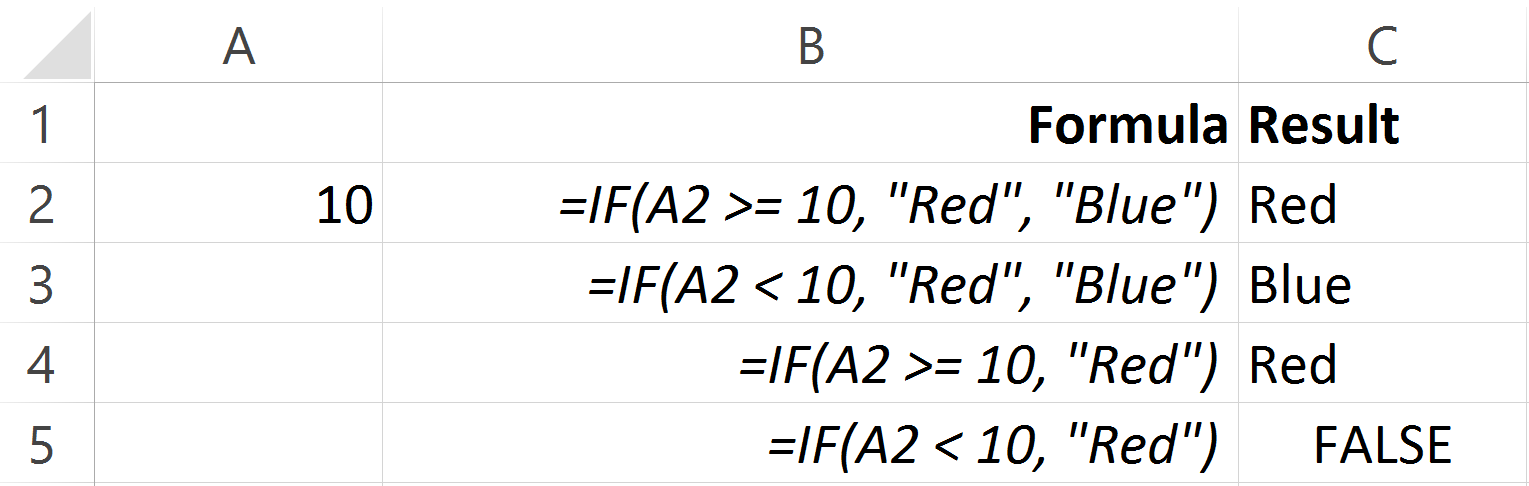
\includegraphics[width=.5\textwidth]{ifExample}
		\label{fig:ifexample} \caption{Configurations of the IF function} \end{figure}
	
	When the user first approaches the tree for a given top-level function -- that
	is, a function nested within none other -- only a few nodes are visible, as
	shown in figure \ref{fig:startpic}. \par
	
	\begin{figure}[h] \centering 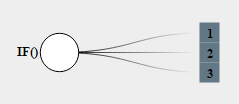
\includegraphics{start} \label{fig:startpic}
		\caption{How the IF tree looks at the start} \end{figure}
	
	The visualization so far comprises two types of node: the circle
	
\includegraphics{glossary-greenonly}, which represents a discrete function in
	the formula and is size according to its frequency relative to the number of
	times to root function appeared\footnote{The root node, by definition, will
		always be the largest node in a tree.}; and the numbered squares
	
\includegraphics{glossary-blue}, which represent the positions of arguments
	within its parent function. From this, we can confirm that, of the times it was
	observed, IF can have at most three arguments passed into it, which corresponds
	with its specifications in the
	API\footnote{https://support.office.com/en-us/article/IF-function-69aed7c9-4e8a-4755-a9bc-aa8bbff73be2}. \par
	
	Knowing that it is the first argument which contains the conditionals, we click
	on the square labeled ``1" to explore. To save space, when more than 10 unique
	arguments have been observed in any position, the tool displays only the first
	ten, with an option to display the rest by clicking the arrow
	
\includegraphics{glossary-arrow}.
	
	\begin{figure}[h] \centering 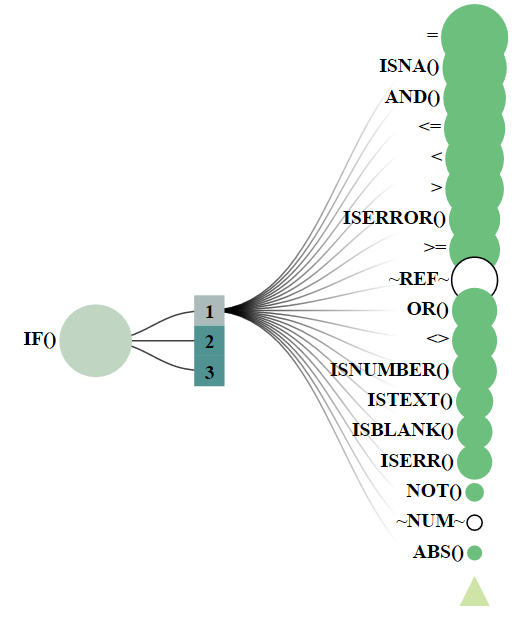
\includegraphics[width=.43\textwidth]{IFexpand}
		\label{fig:expandif} \caption{First argument of the IF tree} \end{figure}
	
	We see that IF contains a number of comparison operators as its first argument,
	such as = and $\le$, and boolean-returning functions, like ISNA and AND, with
	simple equality being the most common and some use as ABS being the least seen
	of everything actually used. \par
	
	From here, we can further explore the common options among these functions.
	Clicking on the ``=" node will yield two arguments and expanding each of them
	will peer into the range of common values of equality comparison, which Figure
	\ref{fig:fullpic} shows. \par
	
	For both sides of the equal sign, the operator has certain types of arguments
	which predominate over the others: on the left side is most often a reference
	to another cell; on the right, a string or number literal, which makes sense
	for the case of confirming a value in another cell before assigning this one.
	Furthermore, a tooltip accompanies each function node in the tree, providing a
	concrete example of a function that uses this structure and where it can be
	found. If this single instance is not enough, then the user also has the option
	to double-click the individual function node, which will open up a new tab with
	a table of many more examples from dataset.
	
	\subsection{Icon Glossary}
	
	From these images, we can provide a quick glossary of images within the
	visualization to aid interpretation. \begin{itemize} \item
		
\includegraphics{glossary-green} - \textbf{Function nodes} are green circles
		labeled with the function name. Their size is determined by their relative
		frequency, scaled logarithmically, to the frequency of the root node in the
		tree. They may have any number of arguments, including zero, as determined by
		the API.
		
		\item \vspace{.25cm}
\includegraphics{glossary-leaf} - \textbf{Value nodes} are
		white circles with a generic label. They represent elements of a formula which
		are which accept no arguments, like references (A1), ranges
		(A1:A10)\footnote{That is, only if both sides of a references are cell
			references. If either side is a function that returns a cell reference, like
			INDIRECT, then the colon should be a function node.}, numbers, boolean values,
		strings, and errors. Functions with zero arguments, like NOW, however, should
		still be considered function nodes.
		
		\item  \vspace{.25cm} 
\includegraphics{glossary-blue} - \textbf{Argument
			nodes} are dark blue squares labeled with a number. The number is the position
		of an argument within the function in the parent node. In \ref{fig:expandif}
		for example, argument node 1 shows every function or value that was seen in
		the first argument.
		
		\item  \vspace{.25cm} 
\includegraphics{glossary-solidline} - \textbf{Solid
			lines} represent a function's ownership of its various arguments. As such,
		they connect the function nodes to argument nodes.
		
		\item  \vspace{.25cm} 
\includegraphics{glossary-fadingline} - \textbf{Fading
			lines} represent the possibility of an argument position to have several
		different possible functions or values. As such, they connect argument nodes
		to function or value nodes.
		
		\item  \vspace{.25cm} 
\includegraphics{glossary-arrow} - \textbf{Expansion
			arrows} appear within an argument node when there are over 10 possible
		functions or values in an argument position. By default, only the first 10
		will be shown along with this arrow; clicking this will show the rest as well.
		
		\item  \vspace{.25cm} 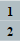
\includegraphics[scale=.75]{glossary-lightblue} -
		\textbf{Optional argument trees} are variations of trees that show only
		formulae with a specific number of arguments, allowing the user to control for
		the presence of optional arguments. By default, trees with dark blue nodes
		contain every type of formula without regard how many arguments they have --
		for example, single-argument ANDs could appear alongside 4-argument ANDs. See
		Figure \ref{fig:optional} to see it visualized. \end{itemize}
	
	\begin{figure}[h] \centering 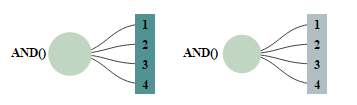
\includegraphics[width =
		.46\textwidth]{comparison} 
\includegraphics[]{comparison-ss}
		\label{fig:optional} \caption{The contents of each type of tree.} \end{figure}
	
	\subsection{Implementation Details} The final visualization is the product of
	two discrete processes: \begin{itemize} \item \textit{Collection}: Given a set
		of Excel sheets, the tool, written in Java, uses Apache
		POI\footnote{https://poi.apache.org/} to identify and iterate over every cell
		containing a valid formula. Afterward, it calls POI's formula parser to break
		the formula text into an ordered set of individual tokens, which the tool then
		parses into the tree-like form. When all formulae have been analyzed like this,
		it produces JSON files for each top-level function in the set.
		
		\item \textit{Presentation}: The JSON files, meanwhile, feed into the
		presentation code, implemented in Javascript with much help from the
		visualization library D3\footnote{https://d3js.org/}. We chose D3 primarily
		for its accessibility: given the JSON, the visualization can be simply
		embedded into a webpage accessible through a browser. \end{itemize} A
	demonstration of the tool can be found at
	https://github.com/DeveloperLiberationFront/Excel-Function-Visualizer.
	
	\subsection{Design Decisions} \label{ssec:decisions} Early in the design, we
	chose the tree form for its inherent ability to represent the loose
	parent-children relationship of formulae as functions and their arguments,
	which could be yet more functions. By adapting this structure to accommodate a
	broad range of possibilities for nested functions, the branching factor depends
	alternatively on the number of arguments in a function and the number of
	possible functions observed as an argument in a function. \par
	
	Guided by the goals in section A, we faced a number of decision points, a
	sample of which we describe below, before we arrived at the design shown above.
	\begin{itemize}
		
		%Can I incorporate these again?
		%			\begin{itemize}
		%
		%				\item [1] \textbf{Provide an interactive environment for free
		% exploration.}
		%				There are a lot of data in some of these collections, and the user should
		% be
		%				able to pick for themselves which to explore while ignoring the rest.
		% Furthermore,
		%				this exploration should not be designed around answering one specific
		% question
		%				but rather be open-ended.
		%
		%				\item [!1] \textbf{Do not make judgments about good and bad design.}
		% Though
		%				users may certainly approach the tool with the intention of finding
		% particular
		%				formulae, \toolname will not prioritize any on metrics of good or bad
		%				practice. Rather, it will present them agnostically, referring only to
		%				frequency.
		%
		%				\item [2] \textbf{Emphasize the quantitative patterns in formula
		%					construction.} \toolname should address the questions of how often the
		%				spreadsheet programmers used a certain function and where they used it.
		% In
		%				this way, it must show precise metrics, such as frequency of use and
		% depth
		% of
		%				function nesting, of the dataset it conveys.
		%
		%				\item [!2] \textbf{Do not overwhelm with numbers.} For popular functions
		%				especially, we anticipated some particularly dense trees. Though
		%				everything should be accessible in accordance with Goal 1, we should
		% design
		% in
		%				a way that reduces noise.
		%
		%				\item [3] \textbf{Promote a qualitative understanding of the patterns.}
		%				\toolname should supplement its observations with concrete instances of
		%				relevant formulae from the corpus. Ideally, it should even direct users
		% to
		% the
		%				exact cell in the spreadsheets where the formula was used,
		% contextualizing
		% the
		%				functions.
		%
		%				\item [!3] \textbf{Do not attempt to explain formulae.} Though \toolname
		% tries
		%				to foster understanding by linking pattern to example, it should not
		% provide
		%				a precise description of what a complex formula accomplishes. The tool's
		% user
		%				must infer this on their own.
		%
		%			\end{itemize}
		
		\item \textit{Copied formulae}: Excel allows users to spread a formula over an
		area, repeating the same task in each cell with minor adjustments. Without
		checking for this, the analysis may not reveal the functions most commonly
		used together but rather the formulae most often applied to large areas. To
		combat this, we converted formulae from their native A1 format to the relative
		R1C1, in which copied formulae should be identical, and considered only each
		R1C1 formulae once per worksheet.
		
		\item \textit{Importance of depth}: When a function appears within another,
		should it be analyzed only as a nested function or would it also be valid to
		analyze the nested function on its own? \par
		
		\ \ For example, in the pictured IF function, we found that people often use
		another IF statement as the second or third arguments of the top-level IF. If
		we only consider functions exactly where they're found embedded in the
		formula, then information about the same function -- IF, in this case -- will
		be scattered across different trees with no way to aggregate them. If we
		record every instance of a function by ignoring their context -- that is,
		including an IF embedded within a SUM function in the same node as the
		top-level IF -- then the tool will represent some functions in multiple nodes
		to capture every possible level of nesting. For now, we only include the
		first, with the latter to be added as an option in the future.
		
	\end{itemize}
	
	\section{Case Study} The obvious question to pose to any visualization is this:
	What do the images tell us that the text could not? It is not enough to
	prove that something can be visualized; we must also demonstrate what
	we can be gained from any particular visualization. As such, we raised a few
	tasks in the introduction in which we thought the tool could help: identifying
	places for API improvement, detecting bad smells, and guiding spreadsheet education. To demonstrate the tool's
	applicability, we sought out places in the tree which best exemplify
	these tasks.
	
	\subsection{API Improvement}
	
	\subsection{Bad Smells} Fowler's description of code smells
	\cite{fowler2009refactoring} underscored an important point of code quality:
	between elegant, efficient code and bug-crippled spaghetti, there is a spectrum of code
	designs which, by themselves, are not faulty but nevertheless suggest vulnerabilities in code design. 	
	Since then, researchers have applied these concepts to spreadsheet programming, as 
	discussed in section \ref{related-work}. While some of the smells lie beyond the scope
	of the tool, such as those characterizing inter-worksheet connections, others
	have structures which create distinctive features within the tree, leading to
	easy detection through our visualization: \par
	
	\begin{itemize} 
		
		\item \textit{Multiple Operations}: A single formula comprises numerous
		functions and operators. \cite{hermans2012detecting}. As a result, the formula
		tends to be prohibitively complex. In the visualization, since each nested and
		combined function creates yet another level of depth within the tree, these
		constructions can result in long, horizontal chains of nodes, as seen in
		figure \ref{"fig:longsum"}.
		
		\item \textit{Long Parameter List}: A function uses numerous arguments, making
		it harder to understand \cite{asavametha2012detecting}. This is not a problem
		for many functions which have a limited number of arguments that it accepts. However,
		for functions that accept arguments indefinitely, such as SUM and CONCATENATE, it creates
		tall towers of argument nodes from a single function node.
		
		\item \textit{Conditional Complexity}: A logical function, particularly IF, nests
		several other logical functions inside of it, reducing code readability \cite{hermans2012detecting}. 
		These can be traced manually in the trees for the logical functions. IF, for example,
		will have several more IF function nodes within its second or third arguments, which
		in turn might have more of the same nested within them.
		
	\end{itemize}
	
	\begin{figure*}[h] \centering 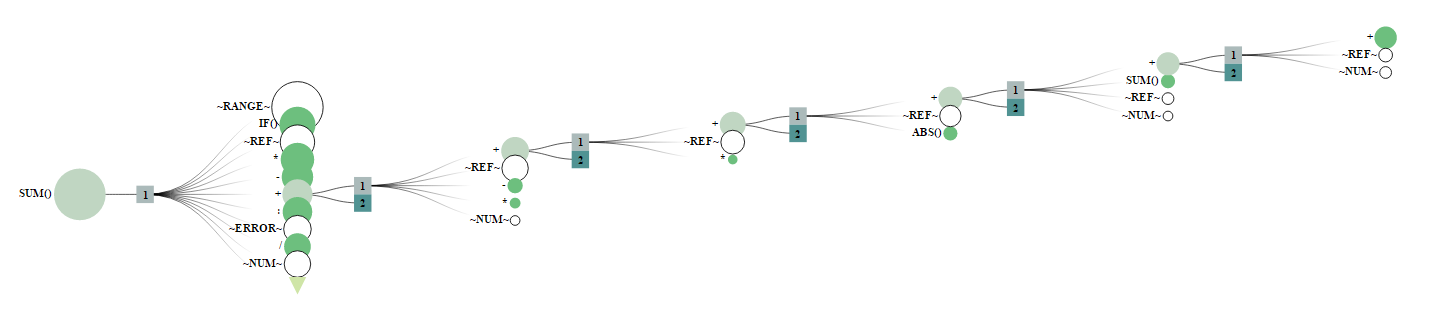
\includegraphics[width=\textwidth]{longsum}
		\label{"fig:longsum"} \caption{The horizontal length of a tree may indicate
			complex or redundant design.} \end{figure*}
	
	Some code issues are meaningful not for the space they occupy but for how they
	clash with a function's expectations. For example, Excel offers a
	number of functions that accept any number arguments given to them, up to a
	resource-defined limit. SUM, for example, simply adds every argument given to it.
	This also means that it can accept only one argument, and when the user does so,
	they pass in a range of cells over 90\% of the time. However, using the tool,
	we isolated an instance where the programmer used a single-argument SUM where the 
	argument was a series of 32 contiguous cells added with the + operation -- 
	``SUM(C6+C7+C8+C9+C10+C11+C12+C13+...+C37)" -- representing a technically
	valid but unusual and problematic design.\par
	
	%Lookup example
	Otherwise, the LOOKUP functions are particularly notorious for their confusing
	mechanisms and, as such, have warranted some especial attention with regards to
	spreadsheet design. In a recent study, Hermans, Aivaloglou, and Jansen probed
	the Enron dataset for uses of VLOOKUP and HLOOKUP specifically. The issue at
	hand was the optional fourth argument: when omitted or set to TRUE, the
	function attempts to return a value from another column by matching two values
	approximately, but when set to FALSE, the match must be exact. Furthermore,
	exact matching works only with sorted columns or rows; if the programmer
	neglects to sort values before calling the *LOOKUP function, they may acquire
	inaccurate results \cite{hermans2015detecting}. \par
	
	Given access to the same dataset, how might this tool approach the issue? On
	the surface, the tool supports easy quantification through the tooltips
	displayed for each node, as shown in figure \ref{fig:vhlookups}, answering the
	question, "How often do spreadsheet programmers use this function?". But, more
	to the point, the tool's distinction between the numbers of arguments for a
	single function lets the user compare frequencies of three-argument forms with
	the four-argument. The visualization does not, however, discern between the
	different values for booleans in the tree, much less whether the spreadsheet
	columns are ordered -- but the linking of examples to patterns allows quick
	insight into which files are at risk for the problems they outlined. \par
	
	\begin{figure}[h] \centering 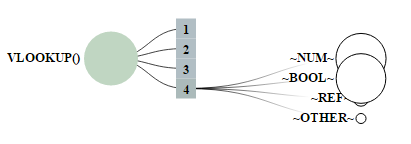
\includegraphics[width=.5\textwidth]{vlookup}
		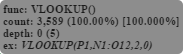
\includegraphics[width=.225\textwidth]{vlookupbox}
		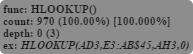
\includegraphics[width=.225\textwidth]{hlookupbox}
		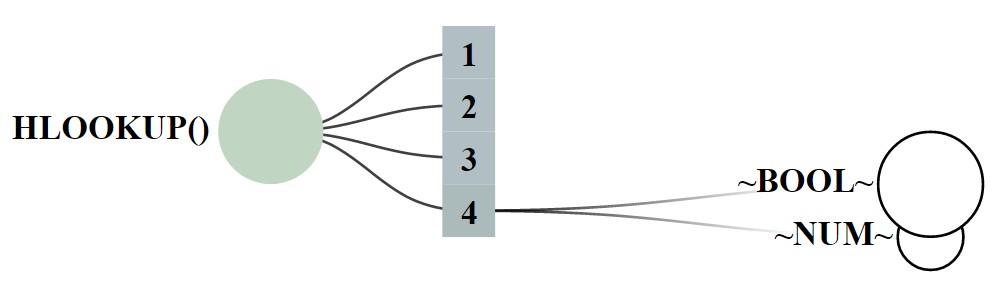
\includegraphics[width=.5\textwidth]{hlookup} \label{fig:vhlookups}
		\caption{VLOOKUP and HLOOKUP with four arguments. Numbers not expected to
			correspond perfectly with \cite{hermans2015detecting}.} \end{figure}
	
	Also at hand are issues with the standard LOOKUP function. Unlike the two
	variations above, LOOKUP accepts either two or three arguments, depending on
	which API-defined form the programmer uses: the vector form or the array form,
	the primary difference being whether the second parameter is a one-column/-row
	range or a two-dimensional array. The array form, as it happens, is strongly
	discouraged by the API in favor of the V/HLOOKUP, a notion that might also be
	leveraged in the pursuit in good spreadsheet design.
	
	\begin{figure}[h] \centering 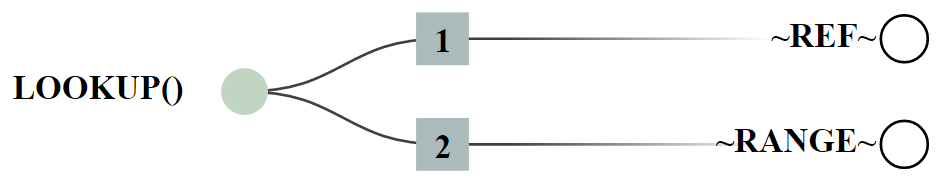
\includegraphics[width=.5\textwidth]{lookup-2}
		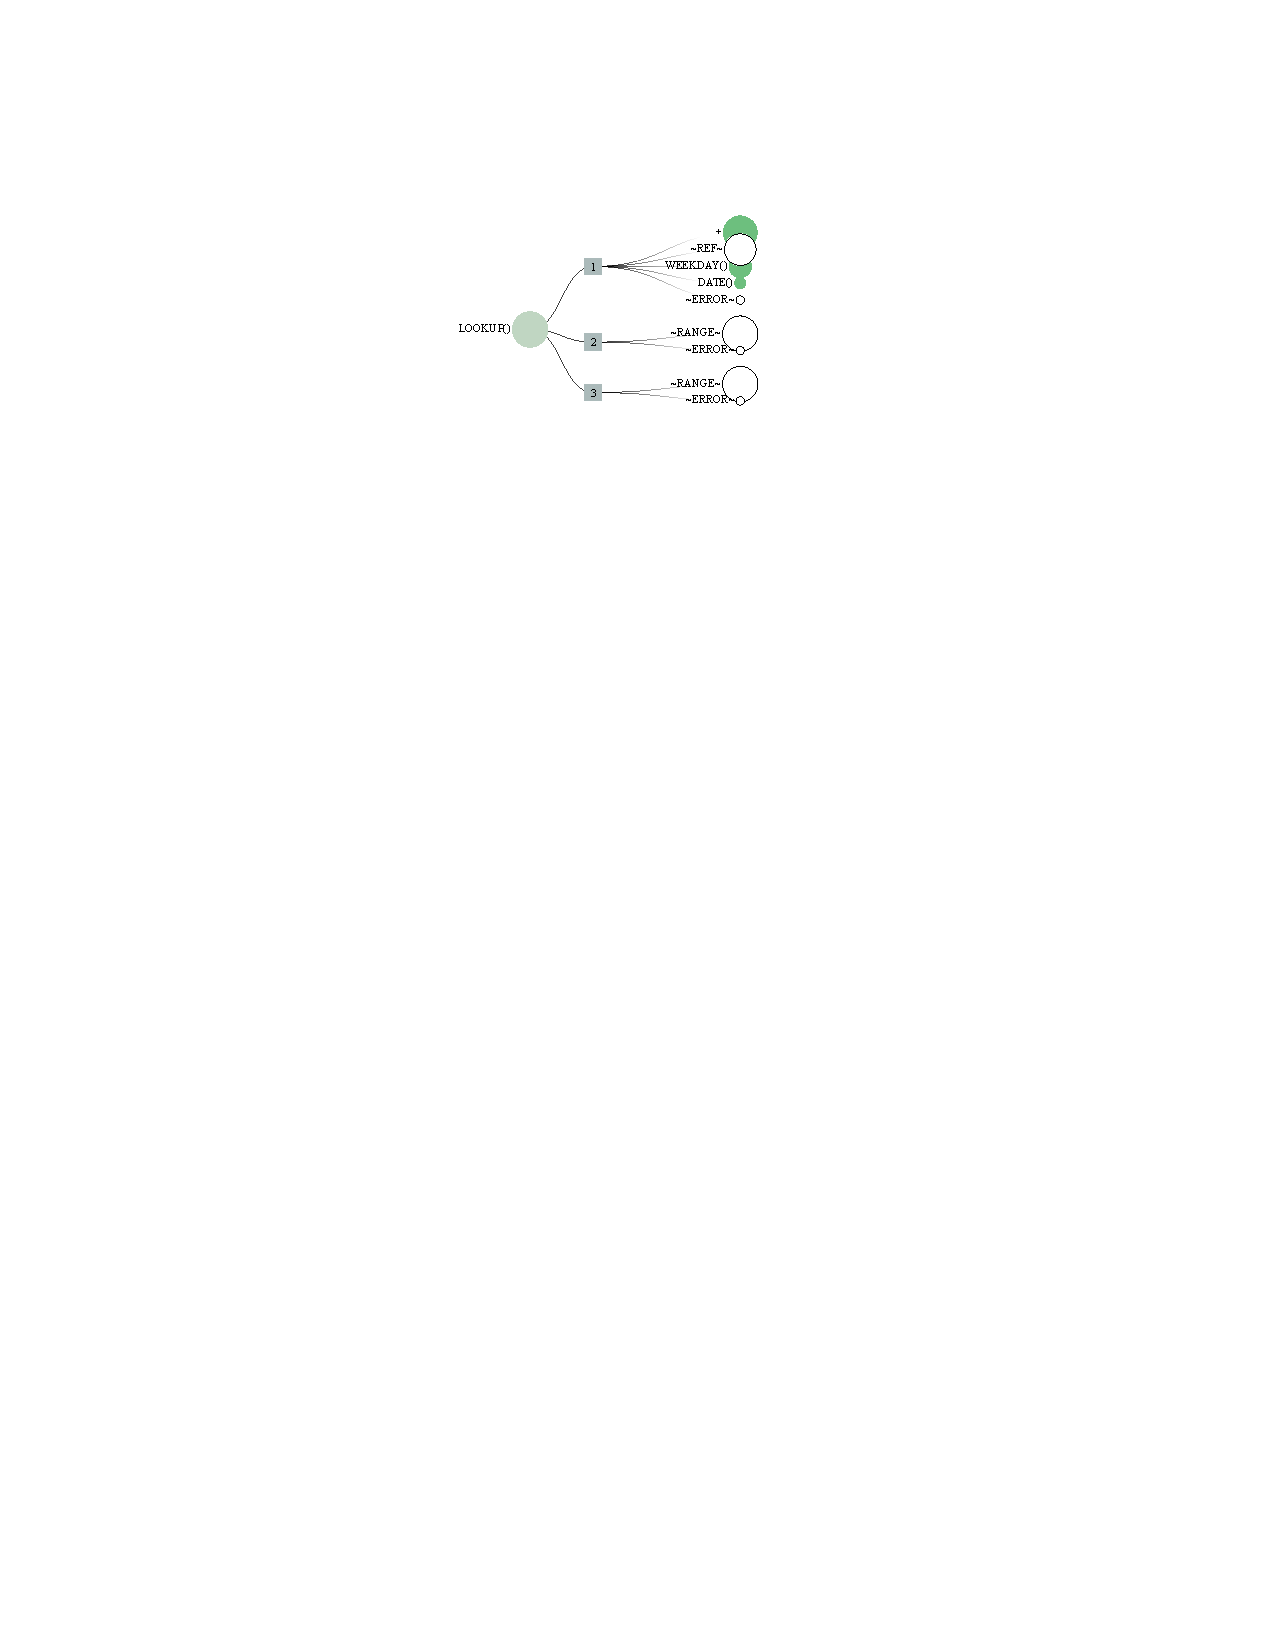
\includegraphics[width=.5\textwidth]{lookup-3} \label{fig:lookups}
		\caption{LOOKUP with two (6 occurrences) and three (1648) arguments.}
	\end{figure}
	
	\subsection{Education} Learning by example has long been a cornerstone of
	effective teacher techniques: by showing the student a concrete example of
	something, rather than dwelling in the realm of abstract description,
	comprehension increases [I'm sure there's a cite out there somewhere.] This is
	no different in software, where every explanation of a tricky programming
	concept is much untangled by the illustrative stub. Even APIs, researchers have
	found, by the inclusion of an in-practice example of the function described.
	Spreadsheet programming, then, should not be essentially different: examples of
	spreadsheet functions in use
	
	\section{User Study} During development, we conducted a brief, four-participant
	user study in order to detect conflicts between our design and the goals in
	section \ref{goals}. We designed the study to be exploratory; given trees based
	in the Enron dataset and at least twenty minutes, we asked the participants to
	adopt the persona of a consultant evaluating a company's spreadsheet
	practice, allowing for questions like which functions on which the employees
	most depended or which sheets or employees presented the most anomalous or
	dangerous designs. Though we instructed them on how to use the tool and
	suggested that they visit one of the most populous trees in the set, we put
	aside any specific tasks or questions and let them choose their own paths.
	Though interpretation of the phrase ``spreadsheet practice" can certainly vary
	from participant to participant, we readily accepted this interpretive
	flexibility since we wanted a range of views and backgrounds despite the
	persona. We clarified, furthermore, that their observations could be directed either at the
	quality of the data conveyed by the tool or at the tool's design itself. \par
	
	Nevertheless, these user studies were a formative moment in evaluating the
	tool's performance, generating a number of directions or corrections in the
	process. We present an overview of responses below, with the four participants
	recorded simply as P1 through P4. \par
	
	\subsection{Use in Smell Tracking}
	\begin{wrapfigure}{O}{.25\textwidth} \centering 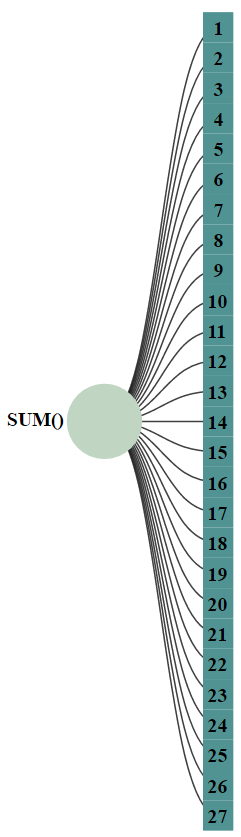
\includegraphics{SUM}
		\label{fig:sum} \caption{An abundance of parameters in SUM} \end{wrapfigure}
	
	The discovery of errors and bad design, whether by purpose or accident,
	produced the more jarring events of the study, and as such, most users
	commented on the tool's ability to locate these problems in spreadsheet design.
	This was often supported by the distinctive visual signatures of certain bad
	practices: multiple arguments produce towers of nodes, deep function nesting
	stretches the tree horizontally, and so on. As such, the participants remarked
	on the problems quickly after opening: P3, exploring the example for a
	27-argument SUM (with SUM's initial appearance pictured left), diagnosed the
	situation with either incompetency or just plain weirdness; P2, meanwhile,
	decided that the spreadsheet's author "was having a bad day" when writing an
	AVERAGE with 18 distinct arguments. Aside from these implicit cues, there are
	also nodes which refer to formula errors, prefixed with \#s, which P4 said
	could be useful if marked well. Furthermore, once these errors are found, the
	participants could then open the offending spreadsheets, discovering that, even
	in context, some of these formulae remained incomprehensible, posing problems
	for the spreadsheet transfer scenarios as outlined by Hermans
	\cite{hermans2011supporting}. The tool, then, aggregates these issues in a
	single place, accessible to either the unguided user and the ones who know
	exactly where to find these issues. \par
	
	The detection of bad design, however, is certainly not limited to a
	visualization tool, and some users remarked that a tool which printed a list of
	errors could suffice just as well for that purpose. However, they also remarked
	that this visual interface better supports the case when searching for new and
	unknown brands of bad smell.
		
	Because the exploratory design makes no qualitative judgment and visualizes
	benign designs with the problematic, it therefore allows for flexible
	interpretation of what is an issue; that is, a user might not realize a certain
	design is suboptimal until they see it in the tree and, at the point, find
	every instance of it.
	
	\subsection{Use in Education}
	The inclusion of formula examples, grounded in
	and linking back to the originating spreadsheets, proved to be an especial draw
	to the tool. After all, none of the participants professed themselves to be
	experts with Excel, their self-reported proficiencies ranging from "fairly
	familiar" (P2) to "not extremely familiar" (P4); even if they were experts, it
	would likely be unreasonable to expect an evenly distributed familiarity with
	the 100+ function trees available. Nevertheless, the list of actual formulae
	accessible through a node's double-click allowed the users a way to find
	examples of formulae with exactly the configuration they wanted. For example,
	as P1 explored the VLOOKUP function, even though they knew the official API
	more verbosely explained its signature, they said they could use the tool to
	collect more examples than the documentation offers. \par
	
	Furthermore, it offers a simple way of finding examples where certain functions
	were used together. though a standard text-search tool might yield the same
	results for a function alone, combinations can require more complex text
	queries, whereas here, the information is already captured in nodes. [This
	paragraph contrasts it with previous approaches, but lacks compelling evidence
	-- a lot of "mights"] \par
	
	Furthermore, just because a user can exhaustively explore every variation of
	how a function was used doesn't mean they will learn exactly what it does. P1,
	in their exploration, examined functions that they hadn't used before, such as
	KURT and PV, and described precisely what types of arguments it accepted and
	how many. However, even after exploring the spreadsheets, they could not
	accurately describe what the functions produced without consulting the official
	documentation. Whether through reticence of the tool or obscurity of the
	functions themselves, the exploratory environment is not enough for independent
	education. However, unlike the previous problem, this can be addressed,
	perhaps, by guiding the user directly to such documentation from within the
	tool without violating any design concerns. \par	

	\subsection{Study Limitations}
	
	Still, several limitations cropped up during the study that complicate the
	evaluation. For one thing, though the source of the data was not explicitly
	stated at the outset of the session, several users studied the file names
	(unchanged as they were) to deduce its roots in finance, if not Enron itself.
	Because of these notorious connotations, then, some were inclined from this
	moment of discovery to orient their exploration around finance-related
	functions, potentially limiting their findings or perceived users for the tool
	-- though some also said that, without this essential context, they could not
	have properly explored a dataset in the first place. Comments like these point
	out the trade-offs of unguided exploration, too: though it might not restrict
	them to a single purpose, it might, at the same time, not afford them any
	mindset at all with which to interpret the data. Another potential problem is
	that the data which users explored was processed and created before we had
	fully completed the tool, meaning some of the counts and patterns in the trees
	were inaccurate. However, we decided that this was not a pressing concern,
	being that we were primarily with whether any interesting reports could be made
	at all, not with whether these reports were 100\% accurate assessments of
	reality. \par
	
	Throughout the study, it became apparent that some of the concepts,
	particularly optional arguments, were easily lost in the representation. To
	illustrate this, consider the following two trees.	
	The difference is, perhaps, too subtle: on the left, the tree contains
	instances of AND functions with any number of arguments, up to four; on the
	right, the tree contains only instances with exactly four arguments. In other
	words, an instance of "=AND(A1, B2, C3, D4)" would be found in both trees,
	while "=AND(A1, B2)" would be found in only the left. Though the users
	naturally did not explicitly report misinterpreting the icons, it became clear
	in their out-loud thoughts that they viewed each box as a fundamentally
	different set of possibilities in formula construction rather than just a
	specific parameter. Though we clarified the meanings when these
	misunderstandings became apparent, these events point to a failure in the tool
	to properly indicate every function with clarity.   \par
		
	
	\section{Limitations} Beyond the negative responses in the user study, a few
	more inherent limitations beset the tool. These largely resulted from
	trade-offs in which we found no acceptable way to win the best of both worlds,
	and necessary compromises were made. \par
	
	Because the data collection depends on POI's formula parser, it affords no
	leeway or partial information from a formula; it either processes it perfectly
	or throws it out. As such, the visualization inhibits insight into anything
	with syntactical errors or third-party functions that can't be evaluated
	without additional tools. Note, however, that this does not include standard
	Excel errors like \#REF! and \#DIV/0, which the parser handles well. This poses
	more egregious problems, however, when POI does not support the parsing of
	certain functions, such as EOMONTH (as obscure as it may be), preventing the
	healthy growth of those trees. \par
	
	Many functions have an expected order of arguments, but some, like SUM and
	MATCH, can be reordered in various ways and maintain their value. However, the
	representation that this tool uses reinforces for all functions that the order
	is important, even in these exceptions. Future work could design a new family
	of tree to accommodate these loose cases, however, by bucketing
	order-insignificant arguments together; this, of course, would still have to
	address the profusion of co-presented data. \par
	
	A larger and related problem is the loss of argument combination. For example,
	figure \ref{fig:index} shows the situation of the INDEX tree, wherein each
	argument position has a few distinct possibilities. While it is easy to break
	down, for each position, which argument types are most common (ranges, MATCH,
	and numbers, respectively), the tree is silent on whether MATCH functions are
	used together in the second and third arguments, among other concerns. Though
	these argument combinations could be pieced together by manually inspecting the
	lists of examples, it is nevertheless inconvenient, though not outside the
	realm of future improvement.
	
	\begin{wrapfigure}{O}{.25\textwidth} 
		\centering 
		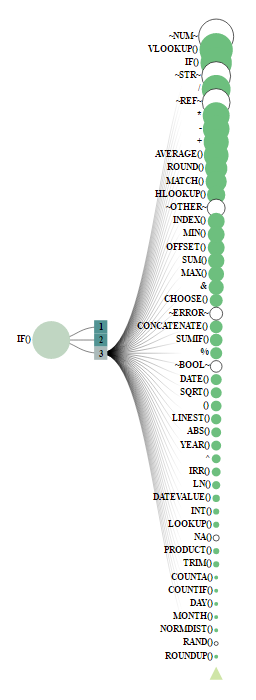
\includegraphics[width=.25\textwidth]{longIF} 
		\label{fig:longif}
		\caption{The many possibilities of IF, argument 3, demonstrate the problem of
			having too many options.} 
	\end{wrapfigure}
	
	A threat to the exploratory philosophy may also mount from the problem of too
	much data, particularly in the popular functions, like SUM and IF. We had added
	some precautions before the study: for any position in the tree, for example,
	only the ten most common functions were displayed without clicking on the
	expansion arrow 
\includegraphics[scale=.35]{arrow}. Nevertheless, P3 remarked
	that they specifically avoided the most popular functions, anticipating a flood
	of nodes from which they could salvage nothing interesting -- which might not
	have been a bad prediction, considering that the SUM is built from 910 nodes
	and IF, at least 18000 [double-check these with refined data]. P2 corroborated
	this by explaining how they gravitated toward specific examples over the plane
	of nodes but complicates it further by also deeming the tool at its best when
	it shows either every possibility of an side-by-side (for comparison) or
	nothing on that branch at all, a balance that is hard to strike with node-dense
	trees. \par
	
	\begin{figure} \centering 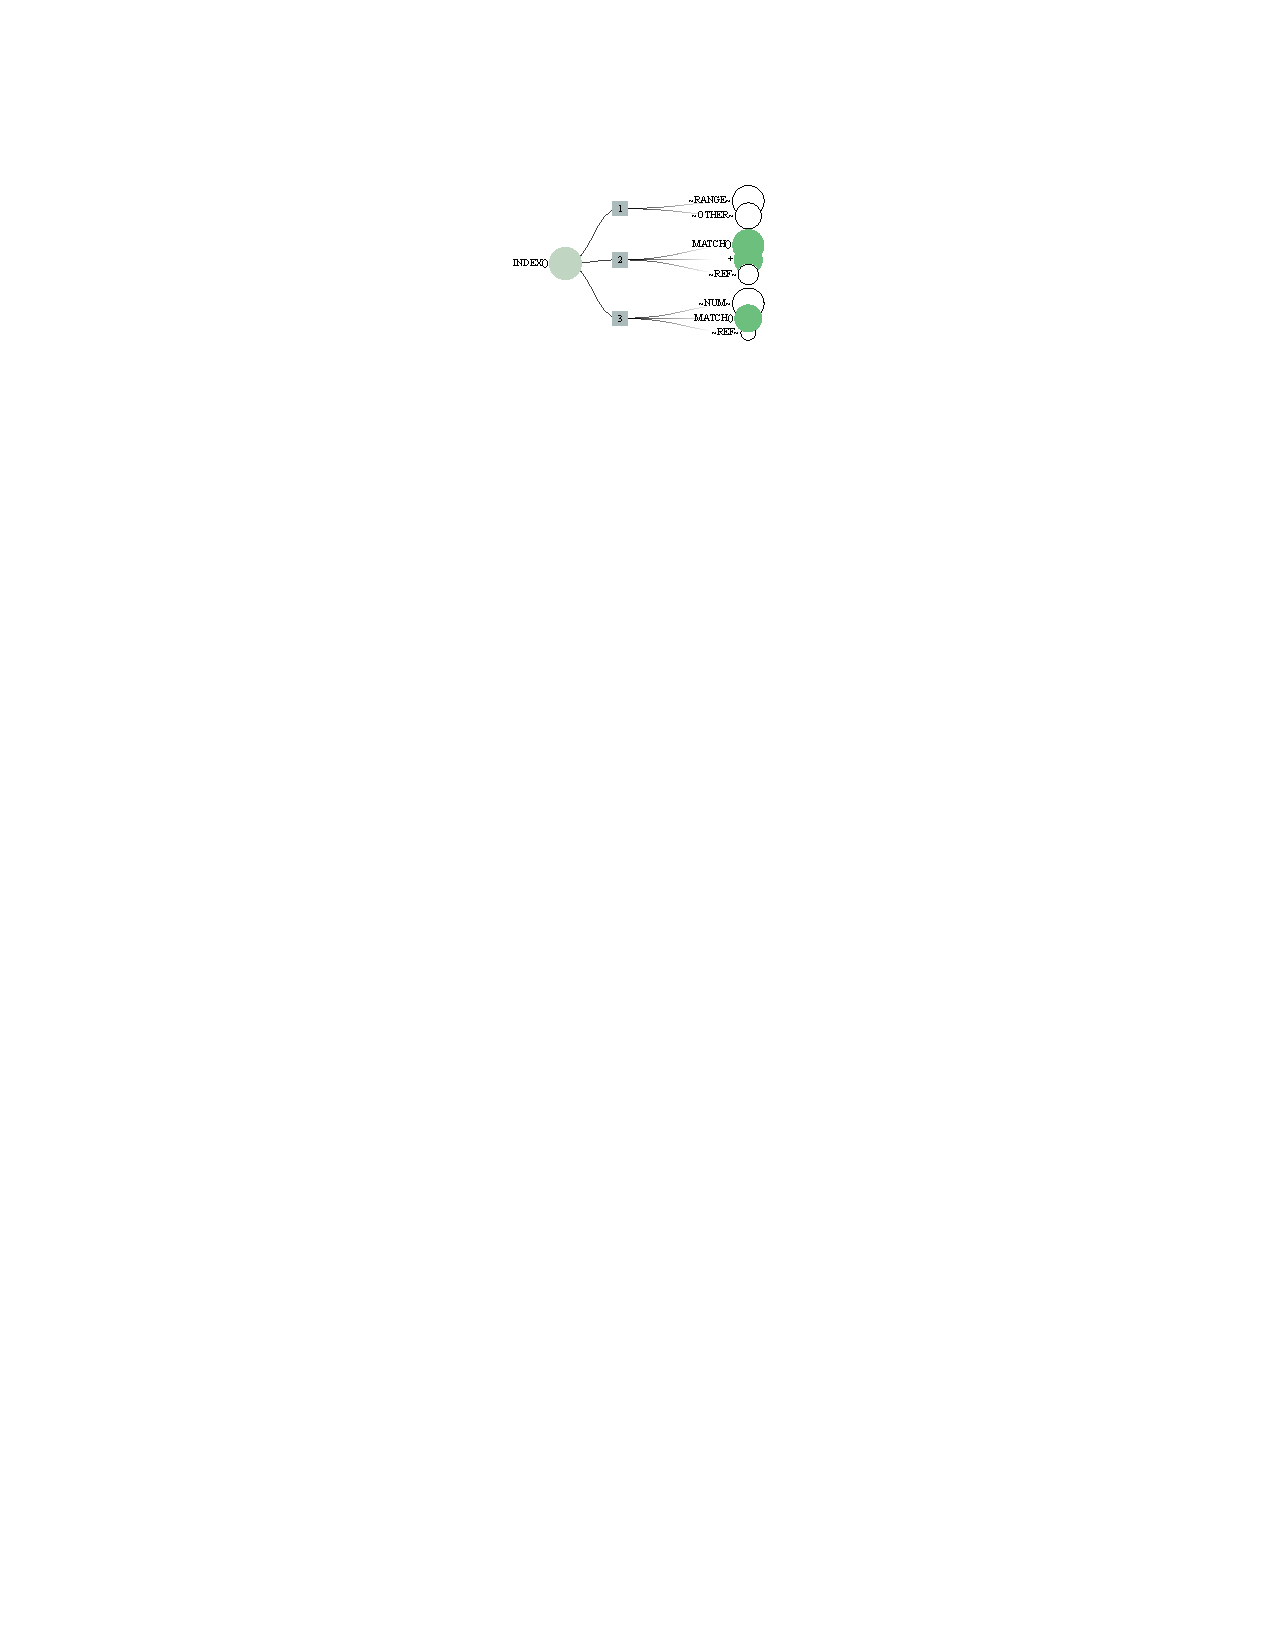
\includegraphics[width=.5\textwidth]{index}
		\label{fig:index} \caption{A difficult question: how often is MATCH used in
			both the second and third arguments?} \end{figure}
	
	%To be sure, though, there is still plenty of work to improve this tool. One
	% activity
	%it does not support well now is that of comparison: for all of it's ability to
	% spit
	%out numbers and quantify patterns,
	
	\section{Future Work} For these user and case studies, we relied solely on
	Enron's spreadsheets to find our results. However, Enron's focus on finances
	and energy represents only one context in which people use spreadsheets. Other
	corpora, like EUSES and Fuse, draw from other domains and industries, and, as
	Jansen found in his comparison of spreadsheets Enron and EUSES, different
	companies rely on different functions. Though the use of a single corpora
	nevertheless suffices for evaluation, we may yet be able to find more
	interesting applications and uses for the tool in other types of spreadsheet.
	\par
	
	Additionally, Excel is only one of many different spreadsheet products
	available, chosen for this project because of its prevalence. But other
	spreadsheets, such as Gnumeric\footnote{http://www.gnumeric.org/} or Google
	Sheets \footnote{https://www.google.com/sheets/about/} represent other
	approaches to spreadsheet systems. Even within identical domains, there's no
	guarantee that practices and functions will hold across these varied offerings.
	This, then, warrants further analysis, in which good visualization might serve
	well. \par
	
	\section{Conclusion} This paper presents a tool to support the exploration of
	function combinations throughout a given spreadsheet dataset. By taking a
	agnostic approach to design quality, it attempts to convey the dataset's
	spreadsheet practices as is: the common along with the anomalous, and the
	well-designed along with the odorous. As seen in the user and case studies,
	this allows it to take on several potential roles at once, such as an
	environment for search out bad code smells as well as a repository for examples
	for learning new techniques. \par
	
	To be sure, we still have a lot of room for improvement. Though the exploratory
	philosophy fostered certain goals well, such as the ability to discover new
	problematic smells without knowing beforehand what they are, it also hindered
	the project in others. Some users, for example, found the trees of popular
	functions to be too crowded to explore well, or that their intention to use the
	tool to examine the good or the bad design exclusively was not fully supported
	by a tool that claimed to know neither. Many of the problems, however, were not
	essential to this design conflict and will be overcome in future iterations of
	design by refining icons and improving maneuverability. \par
	
	Either way, the visualization of these large datasets represents an important
	step in improving practice overall. By taking these voluminous oceans of data
	offered in spreadsheet corpora and rendering them comprehensible through
	images, we seek to draw attention to valuable information that would otherwise
	go unnoticed.
	
	% use section* for acknowledgment
	\section*{Acknowledgment} This material is based upon work supported in whole
	or in part with funding from the Laboratory for Analytic Sciences (LAS). Any
	opinions, findings, conclusions, or recommendations expressed in this material
	are those of the author(s) and do not necessarily reflect the views of the LAS
	and/or any agency or entity of the United States Government.
	
	% references section
	
	% can use a bibliography generated by BibTeX as a .bbl file
	% BibTeX documentation can be easily obtained at:
	% http://mirror.ctan.org/biblio/bibtex/contrib/doc/
	% The IEEEtran BibTeX style support page is at:
	% http://www.michaelshell.org/tex/ieeetran/bibtex/
	\bibliographystyle{IEEEtran} % argument is your BibTeX string definitions and
	% bibliography database(s)
	\bibliography{paper} %
	% <OR> manually copy in the resultant .bbl file
	% set second argument of \begin to the number of references
	% (used to reserve space for the reference number labels box)
	%\begin{thebibliography}{1}
	%
	%\bibitem{IEEEhowto:kopka}
	%H.~Kopka and P.~W. Daly, \emph{A Guide to \LaTeX}, 3rd~ed.\hskip 1em plus
	%  0.5em minus 0.4em\relax Harlow, England: Addison-Wesley, 1999.
	%
	%
	%\end{thebibliography}
	
	
	
	
	% that's all folks
\end{document}


